\section{Intensity Interferometry (II) with IACT arrays}
\begin{figure}
	\centering
	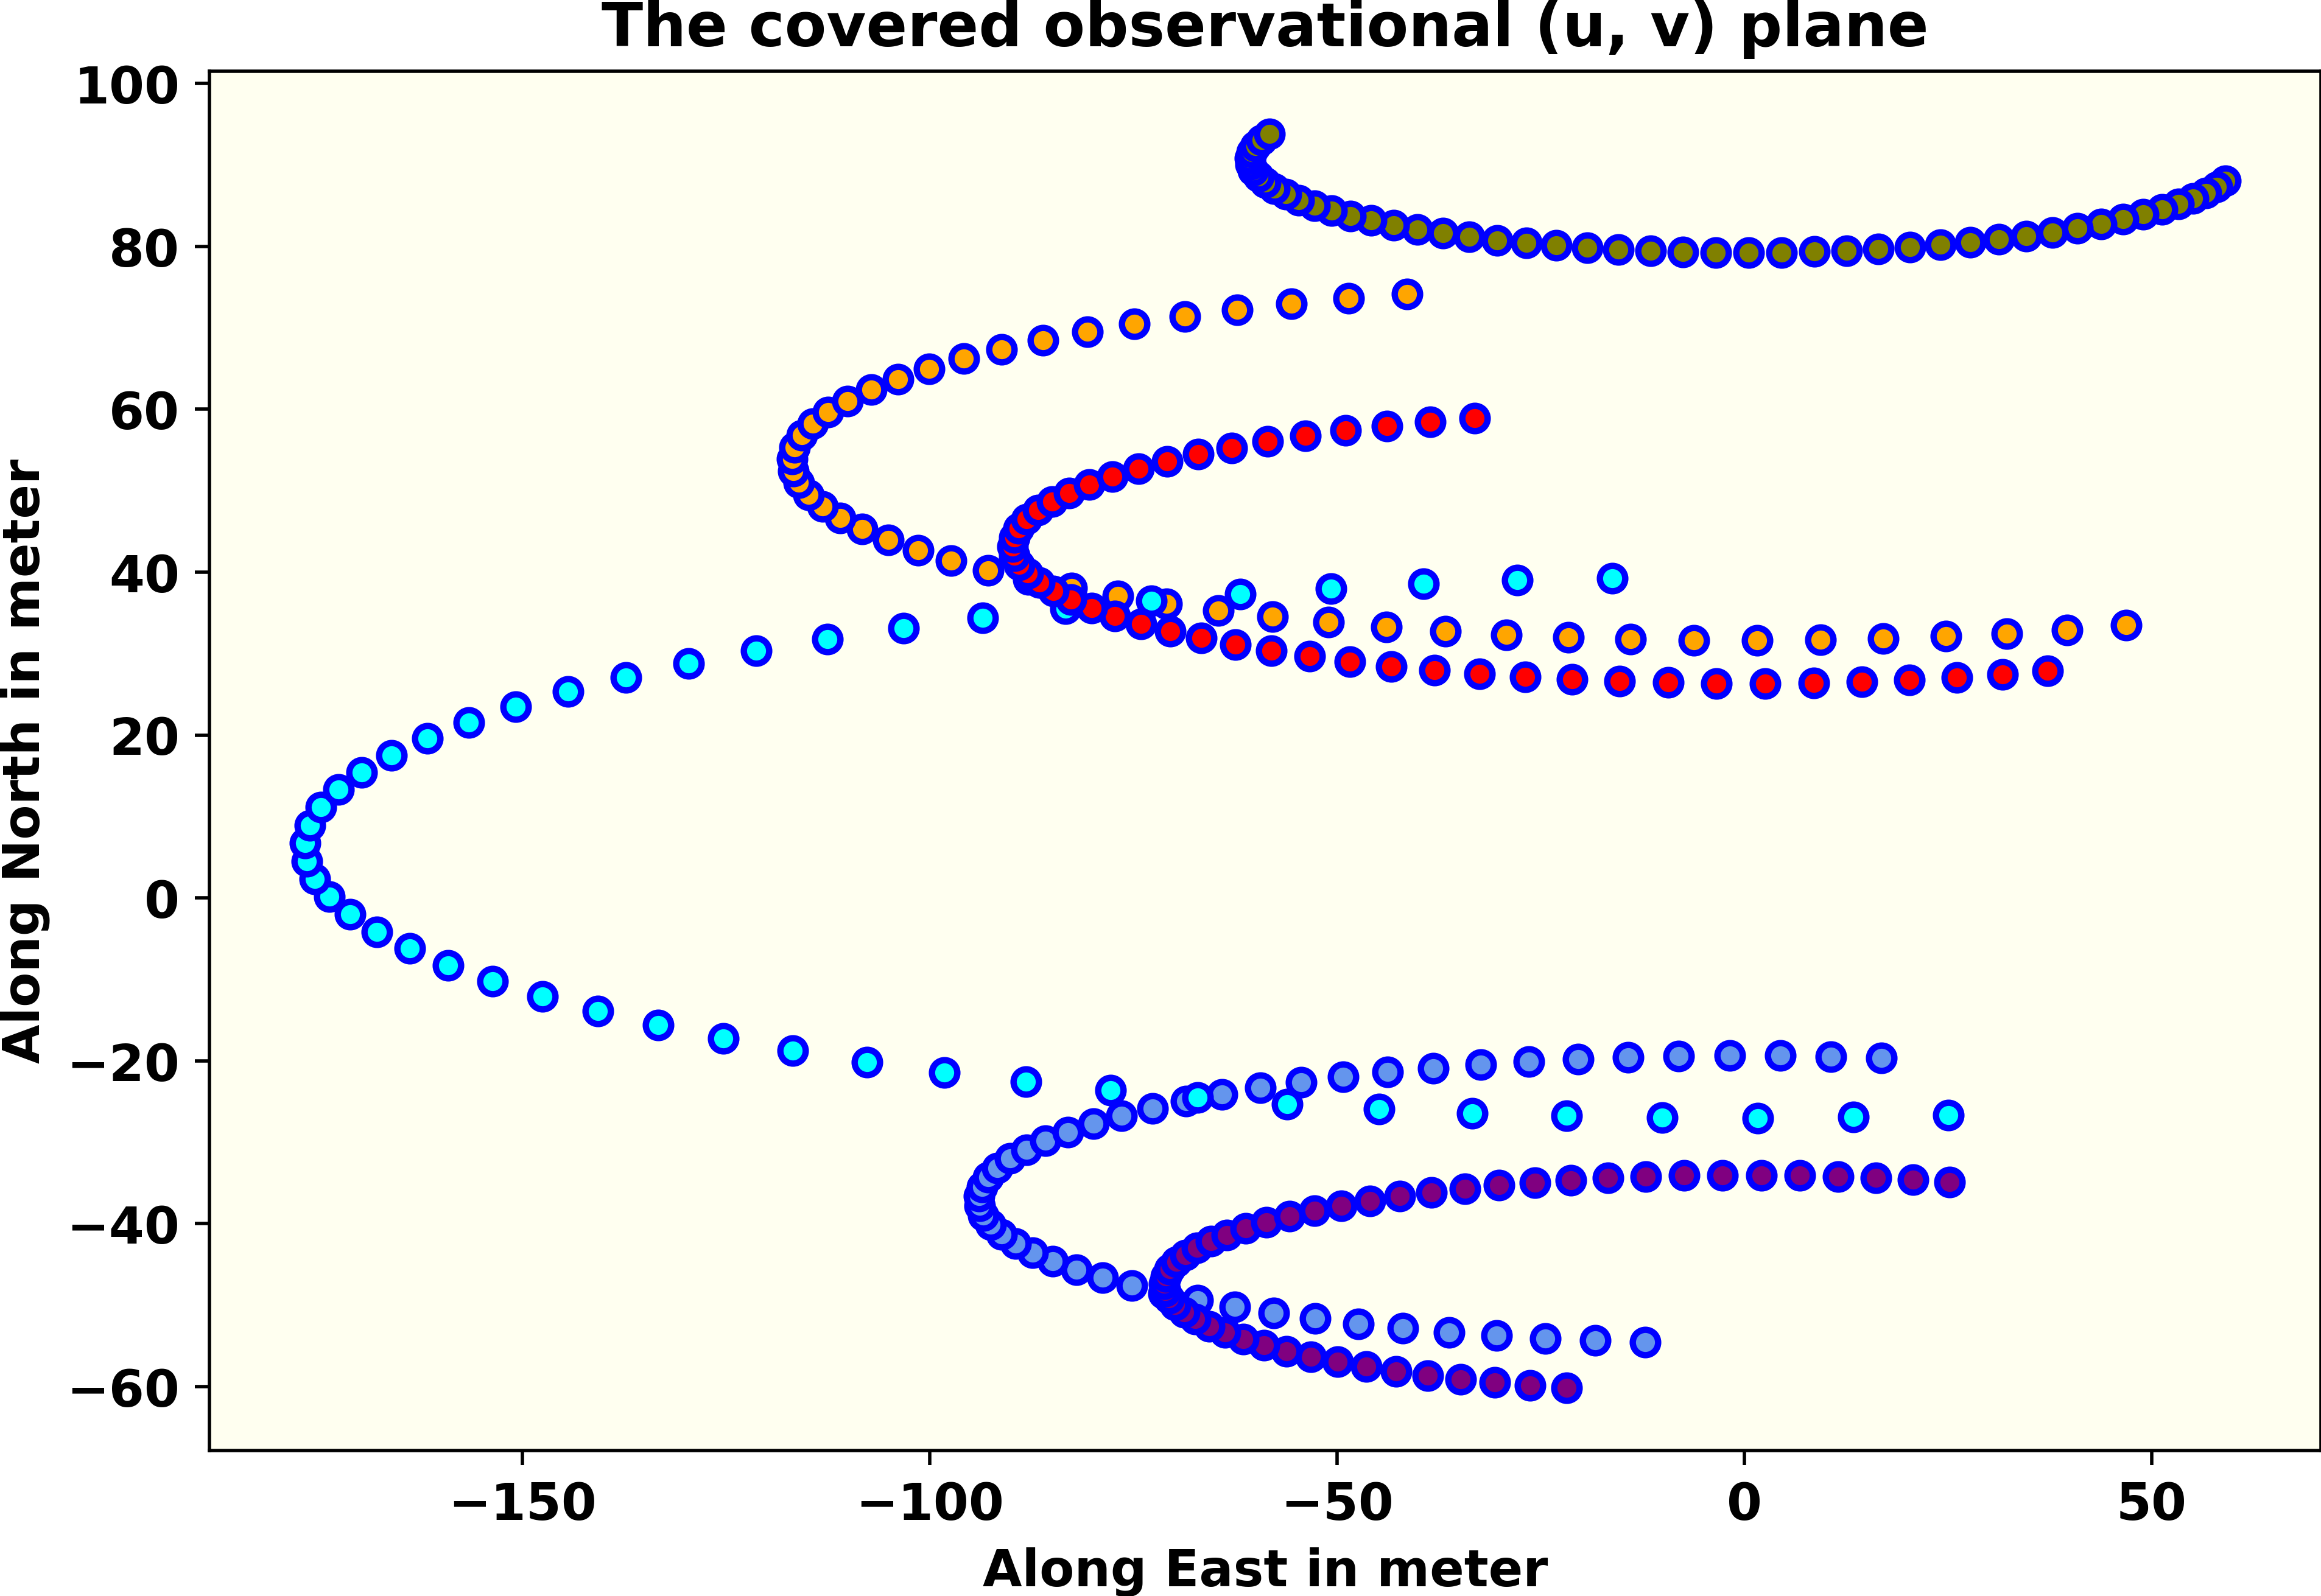
\includegraphics[width=\linewidth]{fig/baseline.png}
	\caption{The tracking of baselines with four telescopes arranged in fig.~\ref{fig:teles} for one night of observation.}
	\label{fig:base}
\end{figure}
\begin{figure}[hbt]
	\centering
	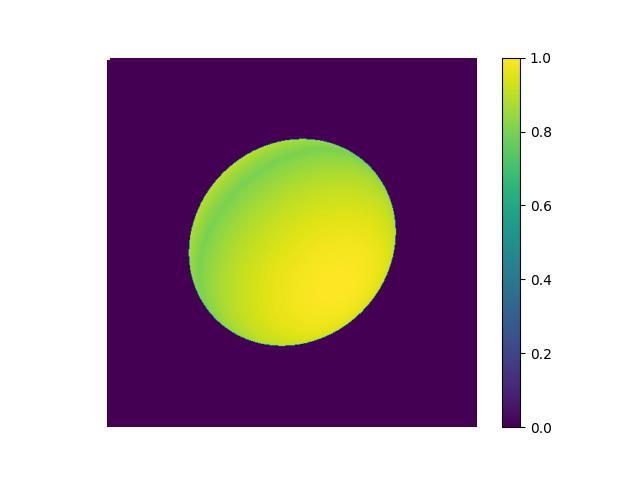
\includegraphics[width=\linewidth]{fig/ellipse/ellipse1612.jpg}
	\caption{This figure shows the simulated fast rotating star. The brightness is highest at the pole and there is gravitational darkening at the equator.}
	\label{fig:image}
\end{figure}
\begin{figure*}
	%\begin{subfigure}{0.5\linewidth}
		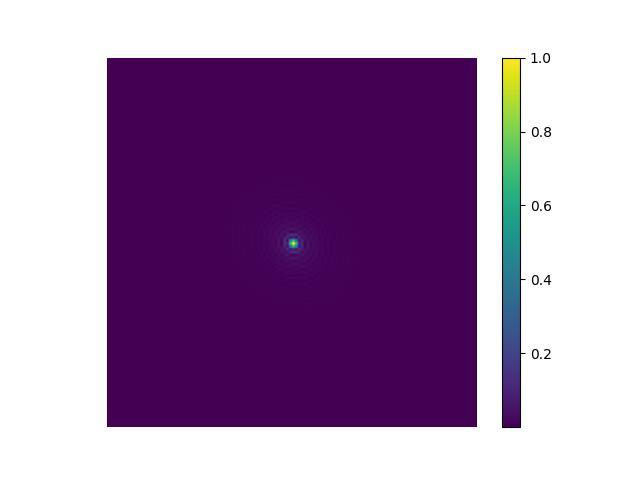
\includegraphics[width=.49\linewidth]{fig/ft/ft.jpg}\hfil
	%\caption{The signal (absolute value of the Fourier transform of the source).}
	%\end{subfigure}\hfill
	%\begin{subfigure}{0.5\linewidth}
		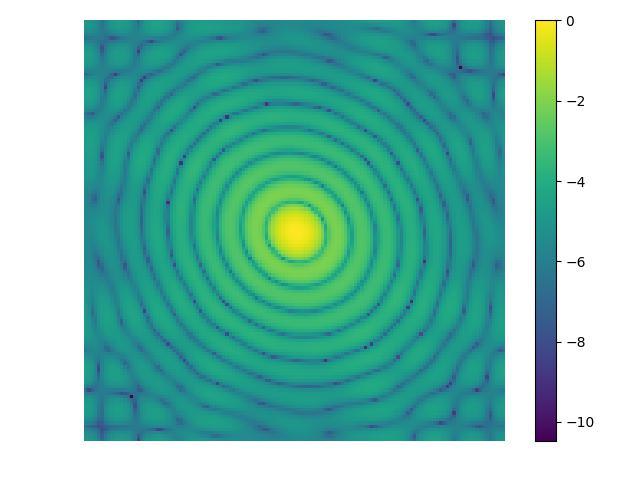
\includegraphics[width=.49\linewidth]{fig/ft/ft_log.jpg}
		%\caption{The logarithm of the signal.}
	%\end{subfigure}
	\caption{Absolute value of the two-dimensional Fast Fourier Transform of Fig.~\ref{fig:image} measured by Intensity Interferometry in the $(u, v)$ plane. \textit{Left.}~Signal on a linear scale. \text{Right}.~Signal on a logarithmic scale.}
	\label{fig:ft}
\end{figure*}
This section presents a brief conceptual overview of how an array of telescopes is used to perform II observations, and explains the Signal-to-Noise Ratio (SNR) from these measurements.
\begin{figure*}
	%\centering
	%\begin{subfigure}{0.5\linewidth}
		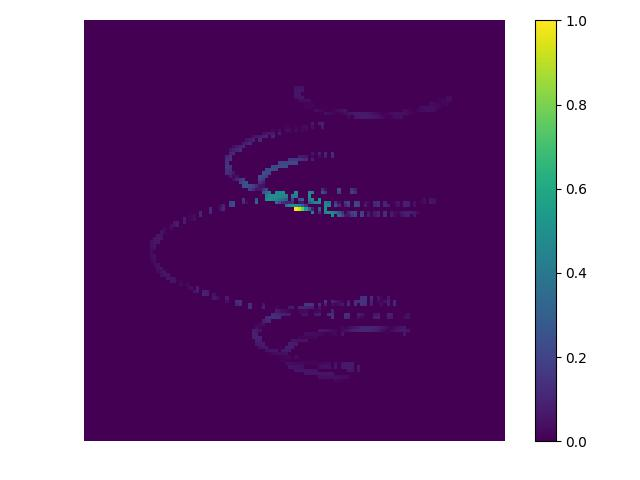
\includegraphics[width=.49\linewidth]{fig/ft/ft_base.jpg}\hfil
		%\caption{The signal as samples by the baselines.}
	%\end{subfigure}\hfill
	%\begin{subfigure}{0.5\linewidth}
		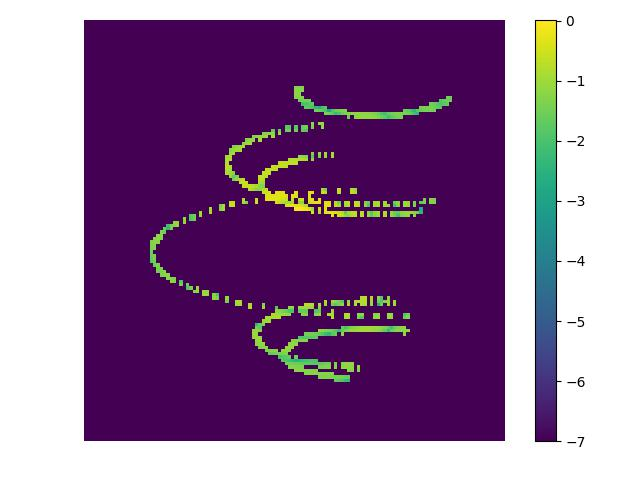
\includegraphics[width=.49\linewidth]{fig/ft/ft_log_base.jpg}
		%\caption{The logarithmic signal as sampled by the baselines.}
	%\end{subfigure}
	\caption{The left panel shows the absolute value of the two-dimensional Fast Fourier Transform of fig.~\ref{fig:image} measured by baselines shown in fig.~\ref{fig:teles}. The right panel shows the same on logarithmic scale}
	\label{fig:ft_base}
\end{figure*}
\subsection{The signal for II}\label{sec:signal}
As a simple example, let us consider a pair of IACTs pointed at a star. Suppose the two telescopes simultaneously measure the intensity of radiation $I_1(t)$ and $I_2(t)$, respectively. The signals from these detectors are cross-correlated and averaged over time, yielding the second order ($n=2$) correlation of these intensities as \citep[cf.][]{acciari2020optical, 2013APh....43..331D}
\begin{equation}
	g^{(2)}= \frac{\left\langle I_1(t) \cdot I_2(t + \tau) \right\rangle}{\langle I_1(t) \rangle \cdot \langle I_2(t) \rangle} 
	\label{eqn:HBT}
\end{equation}
where $\tau$ is the time delay between the telescopes. For spatially coherent and randomly polarized light, eq.~(\ref{eqn:HBT}) reduces to the relation \citep[sometimes called the Siegert relation, see e.g.,][]{acciari2020optical}.
\begin{equation}
	g^{(2)} = 1 + \frac{\Delta f}{\Delta \nu} \abs{V_{12}}^2
	\label{eqn:HBT2}
\end{equation}
where $\Delta f$ is the electronic bandwidth of the photon detectors which measure the intensities.  Values of $\Delta\nu\sim 1\,\mathrm{THz}$ and $\Delta f \sim 1\,\mathrm{GHz}$ are typical of recent work.  In eq.~(\ref{eqn:HBT2}), $V_{12}$, referred to as the complex visibility function, is the Fourier transform of the source brightness distribution. For a uniform disk it is given by
\begin{equation}
 V_{12} = 2 \frac{J_1(\pi\theta_D b)}{(\pi\theta_D b)}
\label{eqn:absvisib}
\end{equation}
where $\theta_D$ is the angular diameter of the star and $b$ is the radial coordinate in the conventional interferometric $(u , v) = (x/\lambda, y/\lambda)$ plane, with $\lambda$ representing the optical wavelength of the filter used for observation. It is evident from eq.~(\ref{eqn:absvisib}) that $V_{12}$ contains information about the star's angular diameter. However, the phase information is lost since we measure only the absolute value $\vert V_{12} \vert^2$. In observational astronomy, the correlation is often expressed in terms of the normalized contrast, given by:
\begin{equation}
	c = \frac{\left\langle \left( I_1(t) - \left\langle I_1 \right\rangle \right) \cdot \left( I_2(t + \tau) - \left\langle I_2 \right\rangle \right) \right\rangle}{\langle I_1(t) \rangle \cdot \langle I_2(t) \rangle} = g^{(2)} - 1
\end{equation}
where, $\left\langle I_1 \right\rangle$ and $\left\langle I_2 \right\rangle$ denote the mean intensities from the two telescopes. Therefore, the signal measured by the photon detector in II, operating with an electronic bandwidth $\Delta f$ within the optical bandwidth $\Delta {\mathrm {\nu}}$ of the observational radiation, is
\begin{equation}
	c = g^{(2)} - 1 = \frac{\Delta f}{\Delta \nu} \abs{V_{12}}^2
	\label{eq:signal}
\end{equation}
$\abs{V_{12}}^2$ is a function of baseline $d = \sqrt{u^2 + v^2}$ on observational plane. Consequently, the strength of the signal is enhanced by employing a large number of baselines.

\subsection{The Signal-to-Noise Ratio for II}
The primary purpose of IACTs is to study high-energy gamma rays (with energy $E\ \geq 30$ GeV) arriving from cosmic sources, entering the Earth's atmosphere, and initiating Cherenkov showers in the upper atmosphere due to multiple scattering. These telescopes feature an array of mirrors that focus light onto a set of photo-multiplier tubes \citep[PMTs, see e.g.,][]{aleksic2016major}. In the simulation model adopted here, we consider a set of four IACTs, each with similar properties. The positional configuration of these IACTs is shown in Fig.~\ref{fig:teles}. The optical signal directed to a PMT is filtered using a spectral filter with a chosen mean observational wavelength $\lambda$ and corresponding bandpass $\Delta \lambda$. The use of filters not only reduces background noise but also improves the signal quality and the efficiency of the PMTs. Filtering background skylight becomes even more significant in II observations, as these are carried out during full moon nights. It is important to note that the light from the stellar source is focused on the PMT during II observations.

The significance of the signal can be expressed in terms of the signal-to-noise ratio (SNR), which depends on many factors. However, most importantly, it does not depend on the optical bandwidth $\Delta {\mathrm {\nu}}$ of the radiation for a two-telescope correlation. The explanation for the independence of the SNR from $\Delta {\mathrm {\nu}}$ is provided in several works \citep[e.g., subsection 4.1 of][]{10.1093/mnras/stab2391}.  The Signal-to-Noise is given by
\begin{equation}
	SNR = A \cdot \alpha \cdot q \cdot n \cdot F^{-1} \cdot \sigma \cdot \sqrt{\frac{T \Delta f}{2}} \cdot \abs{V_{12}}^{2}
	\label{eq:SNR}
\end{equation}
Here, $A$ is the total mirror area, $\alpha$ is the quantum efficiency of the PMTs, $q$ is the throughput of the remaining optics, and $n$ is the differential photon flux from the source. The excess noise factor of the PMTs is represented by $F$, $T$ denotes the observation time, and $\sigma$ is the normalized spectral distribution of the light (including filters) \citep[e.g.,][]{acciari2020optical}. The signal (S) and noise (N) can be understood using eqns.\ref{eq:signal} and \ref{eq:SNR} as:
\begin{equation}
	S = \frac{\Delta f}{\Delta \nu} \abs{V_{12}}^2
\end{equation}
and
\begin{equation}
	N = (A \cdot \alpha \cdot q \cdot n \cdot F \cdot \sigma \cdot \Delta \nu)^{-1}\sqrt{\frac{2 \Delta f}{T}}.
\end{equation}
While most of the parameters can be optimized with hardware, the only way to achieve a better SNR with fixed telescopes is to increase the observation time $T$.

\subsection{Baseline considerations}
The measurement of the size of stellar objects via absolute visibility depends on the distance between the telescopes, known as the baseline $d$.
\begin{equation}
	|V_{12}(d)|^2 = \frac{c(d)}{c(0)}
	\label{eq:angular_size_meas}
\end{equation}
For achieving a good SNR with a given telescope configuration, covering as much as possible of the interferometric plane is always desirable. If the source is at the zenith, the coordinates in the Fourier plane ($u,v$) are given by:
\begin{equation}
	(u,v) = \frac{1}{\lambda} (d_E, d_N)
\end{equation}
where $d_E$ and $d_N$ are the baselines expressed in east and north coordinates. However, of course sources can be anywhere on the sky, and the telescopes are stationary and may also have different relative altitudes $d_A$ depending on the available terrain. Therefore, the Earth's rotation must be taken into account to cover the maximum observational plane using rotated baselines. For a given stellar source with declination $\delta$ and hour-angle $h$, as observed by telescopes at latitude $l$, equation (\ref{eq:baseline_rot}) provides the rotated baselines for a given pair of telescopes \citep[see e.g., eqs.~8--10 from][]{2020MNRAS.498.4577B}.
\begin{equation}
\begin{pmatrix} u\\ v\\ w\\ \end{pmatrix} = R_x(\delta) \cdot R_y(h) \cdot R_x(-l) \begin{pmatrix} d_E \\ d_N \\ d_A \\ \end{pmatrix}
	\label{eq:baseline_rot}
\end{equation}

Fig.~\ref{fig:base} shows the track of six baselines generated from the telescopes (Fig.~\ref{fig:teles}) due to the Earth's rotation. Since every pair of telescopes traces an ellipse in the Fourier plane, the total number of ellipses scales as
\begin{equation}
	\label{eq:N_telescopes}
	\mathcal{N} = \tfrac12 N_T \cdot (N_T -1)
\end{equation}
where $N_T$ is the number of telescopes considered.
As the number of baselines increases non-linearly, Intensity Interferometry (II) benefits greatly from a large number of telescopes. The CTAO can offer many more baselines --- \cite{2013APh....43..331D} considered the telescope configurations then being considered, and all provided dense coverage of the interferometric plane.

\subsection{Fast Rotating Stars: The Objects Considered}
In our work presented here, we simulate a single fast-rotating star to test image reconstruction using a GAN. Fast rotation causes stars to adopt an oblate shape, flattening at the poles and bulging at the equator due to the stronger centrifugal force \citep[e.g.,][]{von1924radiative, 1999A&A...347..185M}. Fig.~\ref{fig:image} shows a fictitious image qualitatively representing a fast-rotating star, with brightness distributed across its surface. The brightness is highest at the poles and lowest at the equator, a phenomenon known as gravity darkening \citep{lucy1967gravity}. This effect was first observed through interferometric and spectroscopic data from the CHARA Array for the fast-rotating star Regulus \cite{mcalister2005first}. Fast-rotating stars are important test cases for understanding various astrophysical processes, including stellar evolution, internal structure, and dynamical behavior over time.

Intensity Interferometry counts the photons arriving at the telescopes from the stellar object. The correlation of these photon arrivals at the telescopes yields the squared visibility Eq.~\eqref{eq:angular_size_meas}, as explained in subsection~\ref{sec:signal}. Fig.\ref{fig:ft} shows the signal from the source shown in Fig.~\ref{fig:image} using II, displayed on both linear and logarithmic scales. In practice, only a small part of this information is available, because one has a finite number of baselines corresponding to the finite number $N_T$ of telescopes at our disposal and a limited observation schedule. Therefore, we have simulated the II observation of a sky source by four telescopes (correlated in pairs) over one night. Using this modest amount of signal from one night's observation, we have trained a cGAN to construct the image of the source.
\begin{figure}
	\centering
	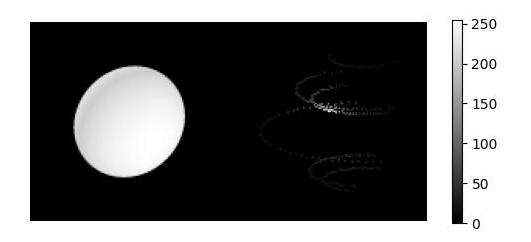
\includegraphics[width=\linewidth]{fig/ellipse1612.jpg}
	\caption{Merged image, which includes the original and the sparsely sampled Fourier plane. It is exactly what the GAN receives. }
	\label{fig:GANinput}
\end{figure}
